\chapter{The ratio of electric field to magnetic field}\label{lec:lec22}
\section{Objectives}
\begin{enumerate}[(i)]
\item To establish the ratio of electric fields to magnetic fields.
\item To identify and explain intrinsic impedance.
\item To identify implications for antenna designs.
\end{enumerate}

Previously we discussed the solution of Maxwell's equation in an unbound medium. We saw that the simplest solution which can exist in the unbound medium is an electric field that is constant in a plane parallel to the direction of the electric field vector or has a variation perpendicular to the direction of the electric field vector. so we assume in previous cases that the electric field was constant in the xy plane. Substituting \={E} in the wave equations, we had a one-dimensional equation $\dv[2]{E_x}{z}$ = $-\omega^2\mu\epsilon E_x$ which was identical to the transmission line equations. 

Then $\frac{d^2E_x}{dz^2}$ + $\beta^2 E_x = 0$ which was a second order differential equation gave $E_x({z}) = E_x^{+}e^{-j\beta z} + E_x^{-}e^{j\beta z}$ as its general solution. This represented two wave traveling in opposite direction +z and -z with amplitude $E_x^{+}$ and $E_x^{-}$. Now we can substitute the solution of the electric field into any of Maxwell's equations to find out the relationship between the electric field and the magnetic field. So we can take the curl equation and substitute the electric field. The electric field is a function of z only, so that

$\frac{d}{dx}$ = $\frac{d}{dy}$ = 0.

%$\hat{y} \frac{d}{dx} E_x^{+} e^{-j \beta z} + %E_x^{-} e^{-j\beta z} = -jw \mu H_x^{x} + H_y^
%{y}$

\begin{dmath*}
\begin{vmatrix}
$\^{x}$ & $\^{y}$ & $\^{z}$\\
0 & 0 & \pdv{}{z}\\
$$E_{x}(z)$$ & 0 & 0
\end{vmatrix} =-j\omega\mu\vec{H} =-j\omega\mu[H_x\hat{x} + H_y\hat{y} + H_z\hat{z}]
\end{dmath*}
where $E_x$ has two components, $E_x^{+}$  $E_x^{-}$

$H_x = H_z = 0$ and so we get only the \^{y} component.\\
\\
$\frac{dE_x(z)}{dz}\hat{y}$ = $\frac{d}{dz}[E_x^+e^{-j\beta z} + E_x^-e^{+j\beta z}]\hat{y}$ = $-j\omega\mu H_y\hat{y}$\\

$-j\beta E_x^+e^{-j\beta z}$ + $j\beta E_x^-e^{-j\beta z}$ = $-j\omega\mu H_y$\\
\\
$H_y = \frac{-j\beta}{-jw\mu}E_x^{+}e^{-j\beta z}$ + $\frac{j\beta}{-jw\mu}E_x^{-}e^{-j\beta z}$

So the magnetic field also has a wave variation in z having two travelling waves. 

$H_y = \frac{\beta}{w\mu}E_x^{+}e^{-j\beta z}$ - $\frac{\beta}{w\mu}E_x^{-}e^{-j\beta z}$

For forward wave, $\frac{E_x^+}{H_y}$ = $\frac{w\mu}{\beta}$, for backward wave 

$\frac{E_x^-}{H_y}$ = $\frac{w\mu}{\beta}$
we substitute for $\beta$ = $w\sqrt{\mu\epsilon}$
\begin{dmath*}
\frac{E_x^+}{H_y} = \frac{w\mu}{\beta} = \frac{w\mu}{w\sqrt{\mu\epsilon}} = {\sqrt{\frac{\mu}{\epsilon}}}
\end{dmath*}
similarly for backward travelling waves,
\begin{dmath*}
\frac{E_x^-}{H_y} = \frac{-w\mu}{\beta} = \frac{-w\mu}{w\sqrt{\mu\epsilon}} = {-\sqrt{\frac{\mu}{\epsilon}}}
\end{dmath*}

it was as if the power was being supplied backward toward the generator. So the negative sign was the reversal of the power flow

Remember the units of $\frac{\mu}{\epsilon}$ = $\frac{H/m}{F/m}$ or $E_x^+$ has V/m and $H_y$ has A/m so that $\frac{\mu}{\epsilon}$ = $\frac{E_x^+}{H_y}$ has unit of impedance $\frac{V/m}{A/m}$ = $\frac{V}{A}$. So whatever the quantity ${\sqrt{\frac{\mu}{\epsilon}}}$ is, it is related to medium parameters of $\mu$ and $\epsilon$ and also has the unit of impedance. So this quantity is similar to what we have got for the transmission line which was characteristic impedance. Then we had the ratio of voltage to current for travelling waves which were characterized by the medium parameters. For wave propagation in 3d space, this property is referred to as INTRINSIC IMPEDANCE of the media denoted by eta $\eta$. $\eta$ = ${+\sqrt{\frac{\mu}{\epsilon}}}$. This quantity plays the same role in the 3d propagation as the characteristics impedance of a transmission line (which is in 1 dimension). So we have a characteristic impedance which is now decided by the medium parameters. If we take a specific case of the medium being free space, $\mu$ = $\mu_{o}$ and $\epsilon$ = $\epsilon_{o}$. So we substitute $\eta$ =$\sqrt{\frac{4\pi \times 10^-7}{\frac{1}{36\pi} \times 10^{-9}}}$, $\eta = 120\pi$ = $\eta_{o}$. So for free space $\eta_{o} = 120\pi$$\Omega$.

When we discuss transmission lines, we saw the ratio of the voltage and current for a travelling wave is always equal to the characteristic impedance same statement we can make for a travelling wave in 3d space, is that for this wave, the ratio of the electric and magnetic field $\frac{E_x^{+}}{H_y}$ or $\frac{E_x^{-}}{H_y}$ is equal to the intrinsic impedance of the medium and for free space, this intrinsic impedance is 120$\pi\Omega$. If we look at a vacuum i.e. free space, the wave seems to see an impedance of $120\pi\Omega$. So a medium like a vacuum or free space appears like an impedance when the wave travels in the medium. Hence free space appears like resistance, which means if the wave travels in it, the wave is essentially delivering power to this medium. So from the perspective of the system generating this wave, it is as if the system is delivering power to space. So space appears like a resistance that consumes power from the system generating the waves. This is interesting because free space is a medium that has nothing in it, yet it appears like a resistance of a value of 377 Ohms. So when we get to discussions on Antennas, we see that space will be treated like an impedance of $377\Omega$ to which power is being delivered. So once we get the intrinsic impedance of a medium, the ratio of electric to the magnetic field is equal to the intrinsic impedance of the medium. This is true for both the forward and backward wave, but however for the backward travelling wave where $\frac{E_x^-}{H_y}$ = - $\sqrt{\frac{\mu}{\epsilon}}$, we recall that we had a similar situation for transmission line also that a backward travelling wave will see an impedance equal to a negative characteristics impedance. We understand that it was as if the power was being supplied backward toward the generator. So the negative sign was the reversal of the power flow and in this case, when we are talking about $E_x$ and $H_y$, we have a negative sign in $\frac{E_x^-}{H_y}$ = -$\sqrt{\frac{\mu}{\epsilon}}$ which also represents the flow of power backward. So for electric and magnetic fields which are perpendicular to each other, E in the x direction and H in the y direction (in this case), For forward travelling wave the ratio of $E_x^+$ to $H_y$ is equal to the intrinsic impedance and if the wave is travelling backward, the ratio is equal to the negative of the intrinsic impedance.

Although we have taken an x-oriented electric field in the case study above, all arguments here will be valid for a y-oriented electric field as far as it is constant on a plane parallel to the direction of the electric field vector. So in general, any electric field oriented in any direction in the xy plane can always be decomposed into the x and y component and then substituted into the equation, and we can find out the relationship between the electric and magnetic fields of the components. So as we did for the analysis for the x-oriented field, if we do the same for the y-oriented field, we again get Expressions similar to that for x-oriented fields.

\={E} = $E_y(z)$\^{y}\hspace{0.15cm} we get\hspace{0.15cm} $\frac{d^2E_y}{dz^2}$ + $\beta^2dE_z$ = 0 and 

$E_y(z) = E_y^+e^{-j\beta z}$ + $E_y^-e^{j\beta z}$

At this point when we find out how $E_y$ relates to H, with the curl $E_x = 0, E_z = 0$ and $\pdv{}{x}$,$\pdv{}{y} = 0$, it varies with z only.

\begin{dmath*}
\begin{vmatrix}
$\^{x}$ & $\^{y}$ & $\^{z}$\\
\frac{\partial}{\partial x} & \frac{\partial}{\partial y} & \frac{\partial}{\partial z}\\
0 & E_y(z) & 0
\end{vmatrix} =
\begin{vmatrix}
$\^{x}$ & $\^{y}$ & $\^{z}$\\
0 & 0 & \frac{\partial}{\partial z}\\
0 & E_y(z) & 0
\end{vmatrix} =-j\omega\mu\vec{H}
\end{dmath*}

Now the magnetic field is not y oriented as the y component is zero.
\begin{dmath*}
-\pdv{E_y(z)}{z}\hat{x} = -j\omega\mu\vec{H} = -jw\mu (H_x\hat{x} + H_y\hat{y} + H_z\hat{z}) 
\end{dmath*}
But	$H_y = H_z = 0$, hence,
\begin{dmath*}
H_x = \frac{1}{-j\omega\mu}\{\frac{-\partial E_y(z)}{\partial z}\} = \frac{1}{jw\mu}\{\frac{\delta E_y(z)}{\partial z}\}
\end{dmath*} 
Recall,
$E_y(z) = E_y^+ e^{-j\beta z} + E_y^- e^{+j\beta z}$
\begin{dmath*}
H_x= \frac{1}{jw\mu} \{-j\beta E_z^+e^{-j\beta z} + j\beta E_z^-e^{+j\beta z} \}
\end{dmath*}
\begin{dmath*}
H_x = - \frac{\beta}{w\mu} E_y^+e^{-j\beta z} +\frac{\beta}{w\mu}E_y^-e^{+j\beta z}
\end{dmath*}
Again we get the two travelling waves for the magnetic field also. Taking the ratio as we have done before; 
For the forward wave,
\begin{dmath*}
\frac{E_y^+}{H_x} = -\frac{w\mu}{\beta} = -\frac{w\mu}{w\sqrt{\mu \epsilon}} = -\sqrt{\frac{\mu}{\epsilon}} = -\eta,
\end{dmath*}
For the backward wave
\begin{dmath*}
\frac{E_y^-}{H_x} = \frac{w\mu}{\beta} = \frac{w\mu}{w\sqrt{\mu \epsilon}} = \sqrt{\frac{\mu}{\epsilon}} = \eta
\end{dmath*}
Notice this is the opposite of what we had seen earlier for the forward and backward waves in terms of the sign of the intrinsic impedance. So when we change the orientation of an electric field, the sign of $\eta$ changes from positive to negative for the forward wave and negative to positive for the backward wave. What this essentially means is that $\frac{E_y^+}{H_x}$ or $\frac{E_y^-}{H_x}$ not only depends on the direction in which the wave is travelling but also on the orientation of the electric and magnetic fields. So we have now E, H and the direction of propagation as a sequence if we follow the right-hand convention and we have E to H in the right sequence i.e $E_x$ and $H_y$ (x to y), then $\frac{E_x^+}{H_y}$ = $+\eta$ and $\frac{E_x^-}{H_y}$ = $-\eta$ but for $E_y$ and $H_x$ (y to x), $\frac{E_x^+}{H_y}$ = $-\eta$ and $\frac{E_x^-}{H_y}$ = $+\eta$ since we are going from y to x which is opposite to the right-hand sequence.

So if E, H, and the direction of propagation follows the sequence x, y, and z directions respectively, then the ratio of $E_x$ to $H_y$ gives a positive intrinsic impedance and the ratio of $E_y$ to $H_x$ gives a negative intrinsic impedance. 

So the electric field(in the x direction) and magnetic field(in the y direction) here are perpendicular to each other and have directions of propagation in the z-direction. That is $E$, $H$ and the direction of propagation are all perpendicular to each other. Hence they form an orthogonal system. Applying the right-hand rule, if we go from E to H in the right-hand sense, then the thumb gives the direction of wave propagation. If we go from the direction of the wave propagation to the direction of the electric field, then the thumb must point in the magnetic field direction.
So if we follow the sequence E, H, and wave direction as x,y, and z respectively, For $\frac{E_x^+}{H_y}$, this is going from x to y and gives a positive sign. Being a forward travelling wave gives another positive sign, so we have a product of two positive signs to get a positive intrinsic impedance ie $(+)(+) = +\eta$. For $\frac{E_x^-}{H_y}$, we have x to y(+), backward wave(-), so $(+)(-) = -\eta$. Similarly, for $\frac{E_y^+}{H_x}$, we are going from y to x(opposite to the right hand convention ie -) and it is a forward wave(+), so $(-)(+) = -\eta$.

So while dealing with these vector fields in 3d space, we consider two things; (i)The orientation of the fields and the sequence, (ii) the direction of the wave propagation. These two together will determine the ratio of electric to magnetic field as being positive $\eta$ or negative $\eta$.

However, the total electric field we are going to see is a resultant of $E_x$ and $E_y$ and $H_x$ and $H_y$ for the magnetic field. So the ratio of the total electric field to the total magnetic field is always a positive value of $\eta$ because,
\begin{center}
$E = \sqrt{E_x^2 + E_y^2}$ and $H = \sqrt{H_x^2 + H_y^2}$
\end{center}
\begin{dmath*}
\frac{|E|}{|H|}=\frac{\sqrt{E_x^2 + E_y^2}}{\sqrt{H_x^2 + H_y^2}} = \frac{\sqrt{\eta ^2H_x^2 + \eta ^2H_y^2}}{\sqrt{H_x^2 + H_y^2}}=\eta
\end{dmath*}

This means that the ratio of the magnitude of the electric field to the magnitude of the magnetic field is always equal to the intrinsic impedance of the medium which is determined by the medium parameters($\mu$ and $\epsilon$).
\begin{center}
Recall, $\eta = \sqrt{\frac{\mu}{\epsilon}}$
\end{center}
So if we know the magnitude of the electric field and the medium parameters, then the magnitude of the magnetic field is uniquely defined. Similarly, if we know the direction of the electric field and the direction of wave propagation, then the direction of the magnetic field is uniquely defined since the electric field, E, magnetic field, H, and the wave propagation are all perpendicular to each other. 
Hence, the magnetic field is completely dependent on the electric field. So we do not have to define the electric and magnetic fields separately.
We can just define the electric field vectorially and the magnetic field should be perpendicular to the electric field and the direction of propagation. This is the reason why whenever we do the wave analysis, we talk only about the electric field as we know that if the electric field is defined, then the magnetic field is automatically defined as the magnetic field is completely dependent on the electric field. We do not have to carry separate information for the magnetic field. Now onward, when we talk about wave propagation in a medium, we describe only the characteristic of the electric field as we can get the characteristics of the magnetic field from the knowledge of the electric field.

So the phenomenon we have discussed up until now describes an electric and magnetic field that are perpendicular to each other and are constant in a plane perpendicular to the direction of propagation of the wave. This phenomenon represents what is called a UNIFORM PLANE WAVE. This wave is a TRANSVERSE ELECTROMAGNETIC UNIFORM PLANE WAVE.

This is the simplest solution that we got for fields in an unbound medium. This was what was investigated before light propagation was understood, and that is what Maxwell showed by analyzing that he got the velocity of light correctly by solving this problem and showing that light is a transverse electromagnetic wave. Since for most of the bulk media, the size of the medium is much larger compared to the wavelength of light, unless you go to structures where the size becomes comparable to the wavelength, we can treat the propagation of light which is an electromagnetic wave like the propagation in an unbound or very large medium. So for that application, the light is treated like a transverse electromagnetic wave. 

But as we will see later if the size of the structure becomes comparable to the wavelength, then the transverse nature of electromagnetic wave is lost and then we have a more complex phenomenon which we will investigate later. So what we have discussed up till now is essentially called PLANE WAVE PROPAGATION OR UNIFORM PLANE WAVE PROPAGATION.

Now if we look at the electric and magnetic fields for plane wave propagation, the analysis shows that the electric and magnetic fields are perpendicular to each other and they are both perpendicular to the direction of wave propagation. The electric and magnetic fields cannot change direction abruptly, they change direction with time so as to keep E and H perpendicular so that the new electric and magnetic field still satisfies the wave equations and Maxwell's equation. The solution which we have got states that E and H must be perpendicular to each other at every instant of time and must be perpendicular to the direction of wave propagation. But the solution did not say what should be the behaviour of the electric and magnetic field as a function of time. In fact, E might change its amplitude as a function of time and the corresponding magnetic field will change its amplitude in exact proportion as a function of time and still satisfy the solution that we have investigated. So in general we can say a uniform plane wave may have electric and magnetic field variations. That is they are uniform in a plane, but the value of the electric and magnetic field at different times may be different. Since we are talking about time-harmonic fields, we can assume that the electric field will be varying sinusoidally i.e. some kind of periodic behavior in electric and magnetic fields. So we have the possibility of E made of $E_x$ and $E_y$ components varying as a function of time and the corresponding H made of $H_x$ and $H_y$ varying as a function of time as well. So we assume that E and H both vary sinusoidally at every instant of time, at every point in space, but E and H remain perpendicular to each other and the ratio of electric to magnetic field is always equal to the intrinsic impedance of the medium. 
Since we are saying that the electric field can vary as a function of time and location in space, if we treat this electric field like a vector i.e. with an arrow to show its direction, with time the top of the arrow will be tracing a curve in the plane perpendicular to the wave propagation

This behaviour will be captured by a parameter called the POLARIZATION of wave. So we define the polarization of the wave as the direction of the electric field or if we treat the electric field like an arrow, the shape which the top of the electric field vector draws on a plane perpendicular to the direction of wave propagation as a function of time. Now we will investigate what is called polarization of uniform plane wave which is a variation of the direction of the electric field and its magnitude as a function of time.

\section{WAVE POLARIZATION}
This is a very important phenomenon in the sense that, any wave you consider will have a direction and magnitude of electric field which in general will vary as a function of time. So every wave will have what is called a state of polarization. Two things might happen when a wave is travelling that is, at any point in space, the electric field vector might change its direction, which we call polarization. Another possibility is that as the wave propagates, at a particular location, the electric field is the same, but as it moves the electric field might change direction. This phenomenon is not polarization, this phenomenon as we will see later is called \textbf{Faraday's Rotation}. So polarization is the orientation of an electric field as a function of time at a given point in space. From point to point, things might change. At a given point in space, we can say that the orientation of the electric field is the polarization of the wave or state of polarization of the wave. So any wave which is generated by a signal will always have a definite polarization. So when we look at this important concept of wave polarization carefully, we see that, since the electric field which propagates in the direction and varies in the xy plane can be oriented in any direction at any instant of time, so we can resolve the electric field into two components or we can generate any arbitrary electric field by a combination of two orthogonal fields; one in the x and the other in the y directions. So we can have $E_x$ and $E_y$ as shown below. 

\begin{figure}[h]
\centering
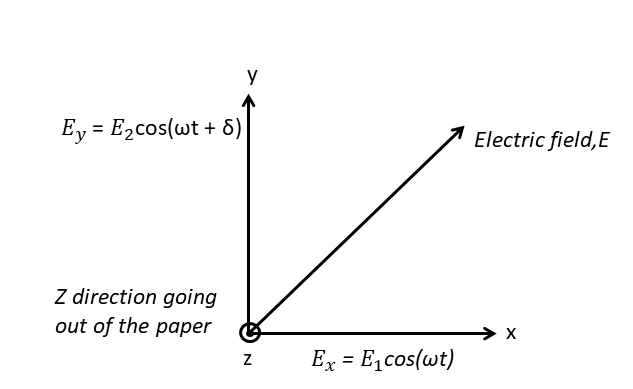
\includegraphics[width=1\linewidth]{\pathtopartone/graphics/E_components}
\caption{electric field vector}
\label{electric field vector components}
\end{figure}
Combining $E_x$ and $E_y$, we can get any arbitrary field in the xy plane where the wave is propagating in the z-direction. So we can combine two sinusoidally varying field $E_x$ and $E_y$, So we have $E_x = E_{1}\cos\omega t$ with $\omega$ as frequency i.e$ E_x = E_{1}\cos\omega t$ oscillates with amplitude going to max $E_{1}$ and min $E_{1}$. So the top of the arrow changes as a function of time.$ E_y = E_{2}(\cos\omega t + \delta)$ in y direction. So we have two fields that are oriented in x and y directions, they have different amplitudes $E_{1}$ and $E_{2}$ and they have a time phase difference $\delta$. If $\delta$ is positive $E_y$ leads $E_x$ and if $\delta$ is negative $E_y$ lags $E_x$. At any instant of time, we have the resultant of $E_x$ and $E_y$ to get $E$. So the shape which E will draw as a function of time represents the state of polarization of that wave that is generated by the combination of the two perpendicularly polarized waves $E_x$ and $E_y$. So if we launch $E_x$ and $E_y$ simultaneously into the medium, at any point in space you get the vector sum $E_x$ and $E_y$ which is E. If we have to determine the locus of the tip of the electric field, then we eliminate the time t in $E_x$ and $E_y$ and then we get the locus of the tip of the electric field vector. That gives the equation of the curve that this particular electric field vector would draw.

$E_x = E_{1}\cos\omega t$ , $E_y = E_{2}\cos(\omega t + \delta)$

$\cos\omega t$ = $\frac{E_x}{E_1}$ and $\sin\omega t$ = $\sqrt{1 - \frac{E_x^2}{E_{1}^2}}$
\\
Recall, $\cos(\omega t + \delta) = \cos\omega t\cos\delta - \sin\omega t\sin\delta$
\\
So,
$E_y = E_{2}\cos\omega t\cos\delta$ - $E_{2}\sin\omega t\sin\delta$

$E_y = E_{2}\frac{E_x}{E_{1}}\cos\delta$ - $E_{2}\sqrt{1 - \frac{E_x^2}{E_{1}^2}}\sin\delta$

$E_y = \frac{E_xE_{2}\cos\delta}{E_{1}}$ - $\frac{E_{2}\sqrt{E_{1}^2 - E_x^2}}{E_{1}}\sin\delta$

$E_yE_{1}$ = $E_xE_{2}\cos\delta$ - $E_{2}\sqrt{E_{1}^2 - E_x^2}\sin\delta$

Hence we have a relationship between $E_{1}$, $E_{2}$, $E_x$ and $E_y$. This will represent the equation of the curve traced by the top of the electric field vector. We shall study the different states of polarization a transverse electromagnetic wave can generate and the implications it has on transmitting the signals efficiently from one point to another. So when we transmit electromagnetic waves, the state of polarization plays a very important role in deciding how much power is transmitted from the system	
